

The lid driven cavity is a famous Computational Fluid Dynamics test case and 
has been studied in countless publications with a wealth of numerical techniques
(see \cite{ertu09} for a succinct review) and also in the laboratory \cite{kost84}.

It models a plane flow of an isothermal isoviscous fluid in a rectangular (usually square) lid-driven cavity. 
The boundary conditions are indicated in the Fig. \ref{fig_ldc}a. The gravity is set to zero.

%---------------------------------------------------------
\subsection{the lid driven cavity problem ({\tt ldc=0})}
In the standard case, the upper side of the cavity moves in its own plane at unit speed, while the other sides are fixed.
This thereby introduces a discontinuity in the boundary conditions at the two upper corners of the cavity and yields
an uncertainty as to which boundary (side or top) the corner points belong to. 
In this version of the code the top corner nodes are considered to be part of the lid. If these are excluded 
the recovered pressure showcases and extremely large checkboard pattern.

This benchmark is usually dicussed in the context of low to very high Reynolds number with the full 
Navier-Stokes equations being solved (with the noticeable exception of \cite{sagl81a,sagl81b,chpc95,eid2005}
which focus on the Stokes equation). 
In the case of the incompressible Stokes flow, 
the absence of inertia renders this problem instantaneous so that only one time step is needed.

%---------------------------------------------------------
\subsection{the lid driven cavity problem - regularisation I ({\tt ldc=1})}

We avoid the top corner nodes issue altogether by  
prescribing the horizontal velocity of the lid as follows: 
\begin{equation}
u(x)=x^2(1-x)^2.
\end{equation}
In this case the velocity and its first derivative is continuous at the corners. This is the so-called regularised lid-driven cavity problem \cite{piva94}.

%---------------------------------------------------------
\subsection{the lid driven cavity problem - regularisation II ({\tt ldc=2})}

Another regularisation was presented in \cite{dejn16}. 
Here, a regularized lid driven cavity is studied which is consistent in the sense that 
${\bm \nabla}\cdot{\bm v}=0$ 
holds also at the corners of the domain.
There are no-slip conditions at the boundaries $x=0$, $x=1$, and $y=0$. 

The velocity at $y=1$ is given by

\begin{eqnarray}
u(x) &=& 1-\frac{1}{4}\left( 1-\cos (\frac{x_1-x}{x_1}\pi)  \right)^2   \quad\quad x\in[0,x_1] \nonumber\\
u(x) &=& 1 \quad\quad x\in[x_1,1-x_1] \nonumber\\
u(x) &=& 1-\frac{1}{4}\left( 1-\cos (\frac{x-(1-x_1)}{x_1}\pi)  \right)^2   \quad\quad x\in[1-x_1,1]
\end{eqnarray}
Results are obtained with $x_1=0.1$.

\begin{center}
\fbox{
\parbox{10cm}{{\bf features}
\begin{itemize}
\item $Q_1\times P_0$ element \index{$Q_1 \times P_0$}
\item incompressible flow
\item penalty formulation \index{penalty formulation}
\item isothermal \index{isothermal}
\item isoviscous \index{isoviscous}
\end{itemize}
}}
\end{center}



\newpage
A 100x100 element grid is used. No-slip boundary conditions are prescribed on sides and
bottom. A zero vertical velocity is prescribed at the top and the exact form of the 
prescribed horizontal velocity is controlled by the {\tt ldc} parameter.

\begin{center}
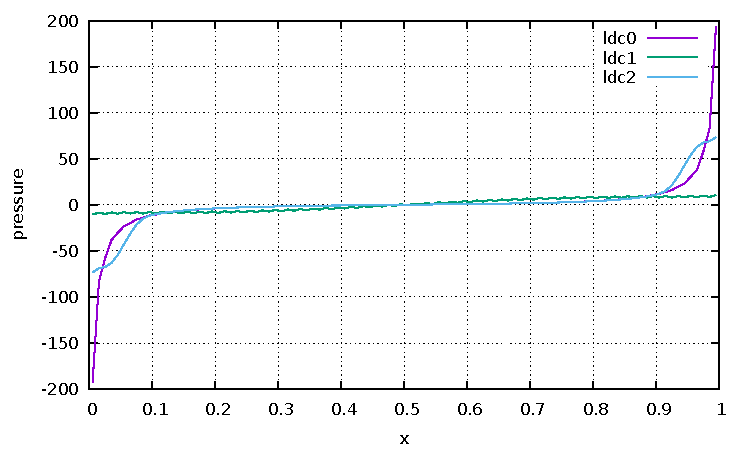
\includegraphics[width=8cm]{python_codes/fieldstone_04/results/p.pdf}\\
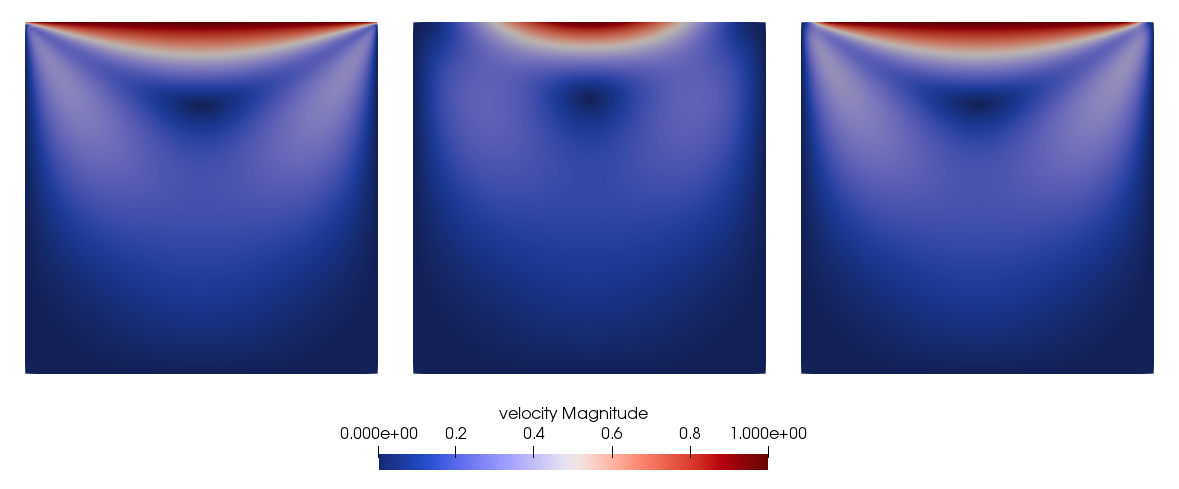
\includegraphics[width=12cm]{python_codes/fieldstone_04/results/velocities}\\
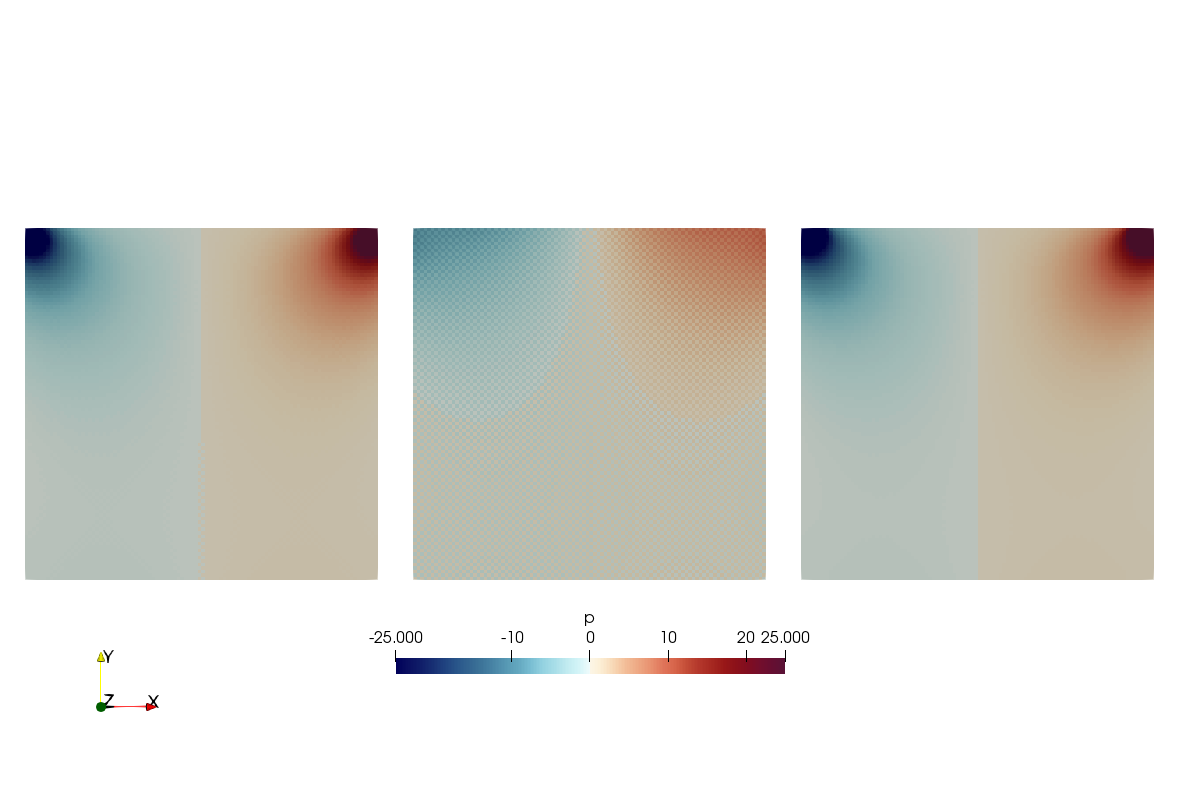
\includegraphics[width=12cm]{python_codes/fieldstone_04/results/pressures}
\end{center}

